\vsb
We now present experiments that were performed using Matlab and an L-BFGS-B
solver~\cite{byrd1995} interfaced by Stephen Becker. Each image is represented by the last map~$\xi^k$ of the CKN, which is used in a linear SVM implemented in the
software package LibLinear~\cite{fan2}. 
These representations are centered, rescaled to have unit~$\ell_2$-norm on
average, and the regularization parameter of the SVM is always selected on a validation
set or by $5$-fold cross-validation in the range~$2^i$,
$i=-15\ldots,15$.

The patches~$\PP_k'$ are typically small; we tried the sizes~$m \times m$
with~$m=3,4,5$ for the first layer, and~$m=2,3$ for the upper ones. The number
of filters~$p_k$ in our experiments is in the set~$\{50,100,200,400,800\}$. The
downsampling factor~$\gamma_k$ is always chosen to be~$2$ between two
consecutive layers, whereas the last layer is downsampled to produce final
maps~$\xi_k$ of a small size---say, $5 \times 5$ or~$4 \times 4$. 
For the gradient map~$\varphi_0$, we approximate the Gaussian kernel
$e^{(1/\sigma_1^2)\|\varphi_0(\z)-\varphi_0'(\z')\|_{\HH_0}}$ by uniformly
sampling~$p_1=12$ orientations, setting~$\sigma_1=2\pi/p_1$.
Finally, we also use a small offset~$\varepsilon$ to prevent numerical
instabilities in the normalization steps~$\tildepsi(\z)= \psi(\z)/\max(\|\psi(\z)\|_2,\varepsilon)$.


\begin{figure}[b!]%lbrt
   \centering
\vs
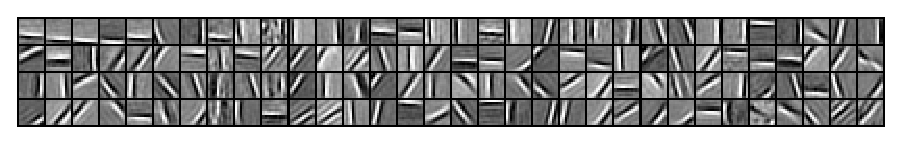
\includegraphics[width=12.5cm]{gabors_final.eps}
\vs
\caption{Filters obtained by the first layer of the convolutional kernel network on natural images.}\label{fig:gabors}
\end{figure}

\vsb
\subsection{Discovering the Structure of Natural Image Patches}\label{sec:gabors}
\vsb
Unsupervised learning was first used for discovering the underlying structure
of natural image patches by Olshausen and Field~\cite{olshausen}.  Without
making any a priori assumption about the data except a parsimony principle, the
method is able to produce small prototypes that resemble Gabor wavelets---that
is, spatially localized oriented basis functions. The results were found
impressive by the scientific community and their work received substantial
attention. It is also known that such results can also be achieved with
CNNs~\cite{ranzato2007}. We show in this section that this is also the case for
convolutional kernel networks, even though they are not explicitly trained to reconstruct
data.

Following~\cite{olshausen}, we randomly select a database of~$300\,000$
whitened natural image patches of size~$12 \times 12$ and learn~$p=256$
filters~$\W$ using the formulation~(\ref{eq:opt}). We initialize~$\W$
with Gaussian random noise without performing the K-means step, in order to ensure that
the output we obtain is not an artifact of the initialization.
In Figure~\ref{fig:gabors}, we display the filters associated to the
top-$128$ largest weights~$\eta_l$. Among the~$256$ filters,~$197$ exhibit
interpretable Gabor-like structures and the rest was less interpretable.
To the best of our knowledge, this is the first time that the explicit kernel
map of the Gaussian kernel for whitened natural image patches is shown to be
related to Gabor wavelets.

\subsection{Digit Classification on MNIST}
The MNIST dataset~\cite{lecun1998} consists of $60\,000$ images of handwritten
digits for training and~$10\,000$ for testing. We use two types of initial
maps in our networks: the ``patch map'', denoted by~CNK-PM and the
``gradient map'', denoted by CNK-GM. We follow the evaluation methodology
of~\cite{ranzato2007} for comparison
when varying the training set size. 
We select the regularization parameter of the SVM by~$5$-fold cross validation when the
training size is smaller than~$20\,000$, or otherwise, we keep~$10\,0000$
examples from the training set for validation.  We report in
Table~\ref{table:mnist} the results obtained for four simple architectures.
CKN-GM1 is the simplest one: its second layer uses $3 \times 3$ patches and
only~$p_2=50$ filters, resulting in a network with~$5\,400$ parameters. Yet, it
achieves an outstanding performance of~$0.58\%$ error on the full dataset.
The best performing, CKN-GM2, is similar to CKN-GM1 but uses $p_2=400$ filters.
When working with raw patches, two layers (CKN-PM2) gives better results than
one layer.  More details about the network architectures are provided in the
supplementary material. In general, our method achieves 
a state-of-the-art accuracy for this task since lower error rates have only
been reported by using data augmentation~\cite{ciresan2012}.

\begin{table}
   \centering
   \renewcommand\tabcolsep{0.16cm}
   \footnotesize
\begin{tabular}{ | c | c |c| c || c | c | c | c || c |c |c|}
\hline
Tr. & CNN & Scat-1 & Scat-2 & CKN-GM1 & CKN-GM2 & CKN-PM1 & CKN-PM2 & \multirow{2}{*}{\cite{zeiler2013}} & \multirow{2}{*}{\cite{goodfellow2013}} & \multirow{2}{*}{\cite{jarrett2009}}  \\
size & \cite{ranzato2007} & \cite{bruna2013} & \cite{bruna2013} & ($12/50$) & ($12/400$) & ($200$) & ($50/200$) &  & & \\
\hline
$300$   & $7.18$ & $4.7$ & $5.6$ & $4.39$ & $4.24$ & $5.98$ & {\bfseries 4.15} & \multicolumn{3}{c|}{NA}\\
$1K$    & $3.21$ & $2.3$ & $2.6$ &   $2.60$ & {\bfseries 2.05} & $3.23$ & $2.76$ & \multicolumn{3}{c|}{NA}\\
$2K$    & $2.53$ & {\bfseries 1.3} & $1.8$ & $1.85$ & $1.51$ & $1.97$ & $2.28$ &  \multicolumn{3}{c|}{NA}\\
$5K$    & $1.52$ & {\bfseries 1.03} & $1.4$ &  $1.41$ & $1.21$ & $1.41$ & $1.56$ &  \multicolumn{3}{c|}{NA}\\
$10K$   & $0.85$ & {\bfseries 0.88} & $1$ & $1.17$ & {\bfseries 0.88} & $1.18$ & $1.10$ &  \multicolumn{3}{c|}{NA}\\
$20K$   & $0.76$ & $0.79$ & {\bfseries 0.58} & $0.89$ & $0.60$ & $0.83$ & $0.77$ &  \multicolumn{3}{c|}{NA}\\
$40K$   & $0.65$ & $0.74$ & $0.53$ & $0.68$ & {\bfseries 0.51} & $0.64$ & $0.58$ &  \multicolumn{3}{c|}{NA}\\
\hline
$60K$   & $0.53$ & $0.70$ & $0.4$ & $0.58$ & {\bfseries 0.39} & $0.63$ & $0.53$ & $0.47$ & $0.45$ & 0.53 \\
\hline
\end{tabular}
\caption{Test error in~$\%$ for various approaches on the MNIST dataset without data augmentation. The numbers in parentheses represent the size~$p_1$ and~$p_2$ of the feature maps at each layer.}\label{table:mnist}
\vs
\vs
\end{table}



\vsb
\subsection{Visual Recognition on CIFAR-10 and STL-10}
We now move to the more challenging datasets
CIFAR-10~\cite{krizhevsky2009} and STL-10~\cite{coates2011}. We select the
best architectures on a validation set of~$10\,000$ examples from the training
set for CIFAR-10, and by~$5$-fold cross-validation on STL-10. We report in Table~\ref{table:cifar} results for CKN-GM,
defined in the previous section, without exploiting color information, and
CKN-PM when working on raw RGB patches whose
mean color is subtracted. The best selected models have always two layers,
with~$800$ filters for the top layer.  Since CKN-PM and CKN-GM exploit a
different information, we also report a combination of such two models, CKN-CO,
by concatenating normalized image representations together. The standard deviations
for STL-10 was always below $0.7\%$.
Our approach appears to be competitive with the state of the
art, especially on STL-10 where only one method does better than ours, despite
the fact that our models only use $2$ layers and require learning few
parameters.
Note that better results than those reported in Table~\ref{table:cifar} have
been obtained in the literature by using either data augmentation (around
$90\%$ on CIFAR-10 for~\cite{goodfellow2013,wan2013}), or external data (around
$70\%$ on STL-10 for~\cite{swersky2013}). We are planning to investigate similar data manipulations
in the future.

\begin{table}[hbtp]
   \centering
   \footnotesize
   \renewcommand\tabcolsep{0.19cm}
   \begin{tabular}{|c||c|c|c|c|c|c|c||c|c|c|}
      \hline
      Method & \cite{coates2011b} & \cite{sohn2012} & \cite{goodfellow2013} & \cite{coates2011} & \cite{bo2013} & \cite{gens2012} & \cite{zeiler2013} & CKN-GM & CKN-PM & CKN-CO\\
      \hline
      CIFAR-10  & 82.0 & 82.2 & \textbf{88.32} & 79.6 & NA   & 83.96 & 84.87& 74.84 & 78.30 & 82.18\\
      \hline
      STL-10  & 60.1 & 58.7 & NA    & 51.5 & \textbf{64.5} & 62.3 & NA& 60.04 & 60.25  & 62.32\\
      \hline
   \end{tabular}
   \vsb
   \caption{Classification accuracy in~$\%$ on CIFAR-10 and STL-10 without data augmentation.}\label{table:cifar}
\end{table}

\vsb
